\section{Experimental Results}
\subsection{Experimental Setup}
\label{sec:setup}
The evaluation uses COCO-$20^i$ and LVIS-$92^i$, derived from COCO~\cite{coco} and LVIS~\cite{lvis}. The author-prepared class memberships comprise four folds of 20 classes and ten folds of 92 classes, respectively~\cite{matcher}. The standard comparison contains 4,000 COCO and 23,000 LVIS episodes per system. A reference cohort varies the demonstration for fixed query targets. A separate component cohort contains 400 COCO and 1,000 LVIS query targets, with up to three references each (1,200 and 2,757 episodes per configuration). All methods within a comparison receive matched inputs.

For each episode, foreground IoU is evaluated at the original query resolution:
\begin{equation}
    J_e=\frac{\mathrm{TP}_e}{\mathrm{TP}_e+\mathrm{FP}_e+\mathrm{FN}_e}.
\end{equation}
The headline metric pools counts within each class, averages classes within each fold, and then averages folds:
\begin{equation}
    J_{\mathrm{fold}}=\frac{1}{F}\sum_{f=1}^{F}\frac{1}{|C_f|}
    \sum_{c\in C_f}\frac{\sum_{e\in E_c}\mathrm{TP}_e}
    {\sum_{e\in E_c}(\mathrm{TP}_e+\mathrm{FP}_e+\mathrm{FN}_e)}.
    \label{eq:pooled}
\end{equation}
Paired comparisons average episodes within each query target $u$ (query image, target mask, and concept), then average the method difference:
\begin{equation}
    \Delta_q=\frac{1}{|U|}\sum_{u\in U}
    \left(\overline J_{u,B}-\overline J_{u,A}\right).
    \label{eq:paired}
\end{equation}
Confidence intervals resample whole query-image clusters, keeping their concepts and references together~\cite{bootstrap,clusterbootstrap}. Exploratory 95\% intervals use 2,000 bootstrap replicates for main/component contrasts and 1,000 for parameter/area analyses. Reference sensitivity is the standard deviation across distinct references after averaging repeated executions of identical inputs. Failed predictions retain missing accuracy; paired contrasts use common successful inputs.

The study covers 36 configurations under a common protocol. Appendix~\ref{app:protocol} gives the full research matrix and implementation details. In comparison tables, bold blue identifies the better value for each metric. In effect tables, blue and coral identify positive and negative effects whose 95\% intervals exclude zero.

\subsection{Accuracy and Efficiency}
% Source: e1_e2_analysis.md, standard cohort and paired comparisons.
\begin{table*}[t]
    \centering
    \small
    \caption{\textbf{Complete-system accuracy.} Class-pooled IoU (\%) and paired equal-query gains (pp; 95\% CI).}
    \label{tab:main}
    \begin{tabularx}{\textwidth}{@{}L{.75}R{.9}R{.6}R{.65}R{2.1}@{}}
        \toprule
        \rowcolor{ReportBlue!12}
        Dataset & Episodes/system & INSID3 & CG-ICS & Paired query effect [95\% CI] \\
        \midrule
        COCO-$20^i$ & 4,000 & 57.65 & \textbf{\textcolor{ReportBlue}{72.17}} & $+14.01$ [$13.16,14.82$] \\
        LVIS-$92^i$ & 23,000 & 40.77 & \textbf{\textcolor{ReportBlue}{47.44}} & $+16.22$ [$15.65,16.82$] \\
        \bottomrule
    \end{tabularx}
\end{table*}

CG-ICS obtains higher accuracy on both datasets (Table~\ref{tab:main}). Its paired equal-query advantage is 14.01 points on COCO and 16.22 on LVIS. The headline class-pooled and paired metrics answer different questions: pooling weights an episode by its predicted/true union within a class, whereas equal-query averaging gives each query target equal weight. On LVIS, CG-ICS's episode-mean IoU is 55.19\%, compared with 47.44\% under mean-fold class pooling. Appendix~\ref{app:math} gives the exact weighting identity behind this distinction.

This accuracy advantage has a substantial computational cost. On exact inputs matched by recorded runner GPU, CG-ICS takes 7.37--10.63 times the mean inference time of INSID3 (Table~\ref{tab:cost}). These times cover inference and exclude model/server startup, evaluation, and output writing. The extra language-model GPU makes the resource difference larger than the runner-latency ratio alone suggests.

% Source: report_inputs_audit/cost_completion.md, exact same-input pairs.
\begin{table*}[t]
    \centering
    \small
    \caption{\textbf{Accuracy--latency trade-off.} Matched-input inference; CG-ICS uses an additional language-model GPU.}
    \label{tab:cost}
    \begin{tabularx}{\textwidth}{@{}L{.65}L{.65}R{.65}R{1.35}R{.7}R{2}@{}}
        \toprule
        \rowcolor{ReportBlue!12}
        Dataset & Runner & Pairs & \shortstack{Mean seconds\\INSID3 / CG-ICS} & Ratio & \shortstack{Episode IoU (\%)\\INSID3 / CG-ICS} \\
        \midrule
        COCO & L40S & 3,095 & \textbf{\textcolor{ReportBlue}{0.454}} / 4.654 & $10.25\times$ & 56.72 / \textbf{\textcolor{ReportBlue}{71.43}} \\
        LVIS & H200 & 3,450 & \textbf{\textcolor{ReportBlue}{0.352}} / 2.595 & $7.37\times$ & 41.97 / \textbf{\textcolor{ReportBlue}{52.28}} \\
        LVIS & L40S & 4,025 & \textbf{\textcolor{ReportBlue}{0.439}} / 4.661 & $10.63\times$ & 40.48 / \textbf{\textcolor{ReportBlue}{54.90}} \\
        \bottomrule
    \end{tabularx}
\end{table*}

The operation counts explain much of this cost: CG-ICS averages 3.43--3.50 language-model requests and 29.89--32.76 SAM calls per standard episode across the recorded hardware strata. Language-model startup adds a median 58--71 seconds, which matters for small batches. Startup and owned-process memory are reported separately in Appendix~\ref{app:cost}.

\subsection{Reference Sensitivity}
% Source: e1_e2_analysis.md, common-success reference statistics.
\begin{table*}[t]
    \centering
    \small
    \caption{\textbf{Reference sensitivity.} Within-query SD ($\downarrow$) and worst-reference IoU ($\uparrow$), in \%.}
    \label{tab:reference}
    \begin{tabularx}{\textwidth}{@{}L{.8}R{1.2}R{.8}R{.8}R{1.2}R{1.2}@{}}
        \toprule
        \rowcolor{ReportBlue!12}
        Dataset & Eligible queries & \shortstack{SD\\INSID3} & \shortstack{SD\\CG-ICS} & \shortstack{Worst IoU\\INSID3} & \shortstack{Worst IoU\\CG-ICS} \\
        \midrule
        COCO & 2,000 & 16.33 & \textbf{\textcolor{ReportBlue}{13.26}} & 14.75 & \textbf{\textcolor{ReportBlue}{26.53}} \\
        LVIS & 4,308 & \textbf{\textcolor{ReportBlue}{13.10}} & 18.79 & 13.97 & \textbf{\textcolor{ReportBlue}{18.34}} \\
        \bottomrule
    \end{tabularx}
\end{table*}

The complete-system accuracy ranking does not determine the variability ranking. CG-ICS reduces reference SD on COCO but increases it on LVIS (Table~\ref{tab:reference}). Nevertheless, its mean worst-reference IoU is higher on both datasets. A system can therefore improve the lower end of observed performance while remaining more sensitive to which reference is chosen.

The same direction appears in H200-only subsets: the CG-ICS minus INSID3 reference-SD interval is $[-3.71,-2.69]$ points on COCO and $[5.03,5.98]$ on LVIS. Reference robustness is therefore dataset-dependent, and reduced variability should be interpreted alongside the achieved accuracy.

A three-seed study fixes the component inputs and yields mean per-input CG-ICS SDs of 2.23 points on COCO and 3.65 on LVIS. Prediction hashes are identical across all three seeds for 263/1,200 and 694/2,757 inputs. These measurements capture sensitivity across executions, including seed and GPU variation.

\subsection{Component Ablations}
INSID3's gains are not explained by the feature trunk alone. Removing debiasing from the full processing route reduces equal-query IoU by 2.38 points on COCO and 2.26 on LVIS. Replacing self-plus-cross aggregation with seed-only output reduces it by 9.24 and 4.06 points, respectively. The full processing route improves over debiased simple similarity by 19.23 and 11.94 points. These contrasts indicate that both the representation adjustment and the use of clustered spatial structure matter.

For CG-ICS, language and visual prompts provide complementary information. Adding visual boxes to a single concept yields 5.39 points on COCO and 4.78 on LVIS; adding a concept to the visual-only system yields 13.38 and 16.54 points. By contrast, the incremental return from more search depends on the dataset and on the already available visual route.

% Source: components_analysis.md paired equal-query contrasts, seed0.
\begin{table*}[t]
    \centering
    \small
    \caption{\textbf{Component effects.} Paired equal-query IoU effects (pp; 95\% CI).}
    \label{tab:components}
    \begin{tabularx}{\textwidth}{@{}Xrr@{}}
        \toprule
        \rowcolor{ReportBlue!12}
        Intervention & COCO effect [95\% CI] & LVIS effect [95\% CI] \\
        \midrule
        INSID3: add debiasing to self/cross & \textcolor{ReportBlue}{\textbf{+2.38}} [$1.25,3.55$] & \textcolor{ReportBlue}{\textbf{+2.26}} [$1.57,2.95$] \\
        INSID3: self/cross instead of seed-only & \textcolor{ReportBlue}{\textbf{+9.24}} [$7.19,11.25$] & \textcolor{ReportBlue}{\textbf{+4.06}} [$3.02,5.18$] \\
        CG-ICS: visual boxes with one concept & \textcolor{ReportBlue}{\textbf{+5.39}} [$3.80,7.00$] & \textcolor{ReportBlue}{\textbf{+4.78}} [$3.63,6.02$] \\
        CG-ICS: search beyond scored candidates, with boxes & $-0.07$ [$-0.78,0.65$] & \textcolor{ReportBlue}{\textbf{+1.45}} [$0.67,2.25$] \\
        \rowcolor{TableTint}
        CG-ICS: full search beyond one concept, with boxes & $+0.22$ [$-0.81,1.29$] & \textcolor{ReportBlue}{\textbf{+2.30}} [$1.38,3.25$] \\
        \bottomrule
    \end{tabularx}
\end{table*}

With visual boxes, full search adds 0.22 points beyond a single concept on COCO, with a confidence interval spanning zero; the corresponding LVIS gain is 2.30 points. Without boxes, the gains rise to 3.07 and 5.30 points. Thus, the observed contribution of search depends on both the dataset and the visual route.

\paragraph{Search--prompt interaction}
Let $J_u(s,v)$ denote reference-averaged IoU for query target $u$, with
$s\in\{0,1\}$ selecting a single concept or full search and
$v\in\{0,1\}$ indicating visual boxes. The interaction contrast is
\begin{equation}
  \begin{aligned}
  \Gamma=\frac{1}{|U|}\sum_{u\in U}\bigl[&J_u(1,1)-J_u(1,0)\\
                              &-J_u(0,1)+J_u(0,0)\bigr].
  \end{aligned}
  \label{eq:search-visual-interaction}
\end{equation}
This measures how much search changes the marginal benefit of visual
prompting. The observed interaction is $-2.85$ percentage points on COCO
(95\% CI $[-4.29,-1.48]$) and $-3.00$ on LVIS
($[-4.09,-1.95]$). Thus, on the full matched input cohort, the two additions
have diminishing joint gains: visual boxes help at both search levels,
but help more when only the initial concept is used.



\begin{figure*}[t]
    \centering
    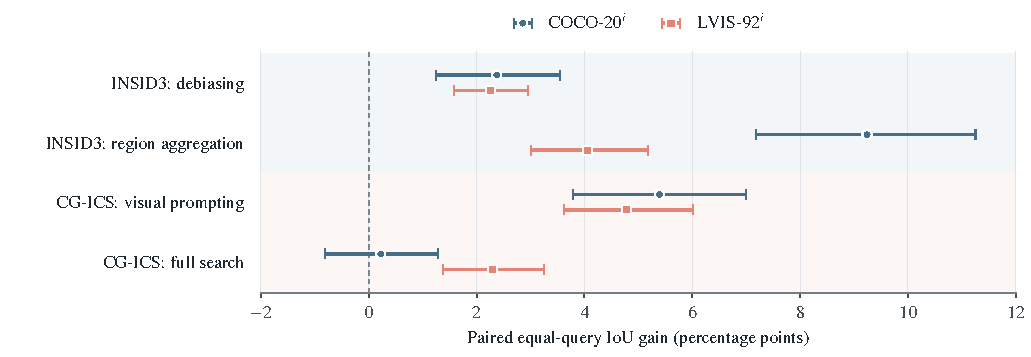
\includegraphics[width=\linewidth]{figures/component_effects.pdf}
    \caption{\textbf{Component gains.} Equal-query IoU effects with 95\% image-cluster confidence intervals.}
    \label{fig:components}
\end{figure*}

The single-concept route is also much cheaper. Full search takes 4.17 times as long on 300 matched COCO/H200 inputs and 4.37--4.56 times as long on matched LVIS subsets. The accuracy changes on those same timing subsets are $-0.54$ points for COCO, $+1.53$ for LVIS/L40S, and $+3.67$ for LVIS/H200. These paired observations motivate input-dependent search (Section~\ref{sec:extension}).

The candidate-stage comparison combines generation and selection, while full search also includes restarts. A fixed-pool ablation can isolate the scoring terms in Eq.~\ref{eq:cg-score}; this control forms part of the evaluation design in Section~\ref{sec:extension}.

\subsection{Feature Backbones}
% Source: components_analysis.md E5 mean-fold mIoU; common1008 input.
\begin{table*}[t]
    \centering
    \small
    \caption{\textbf{Representation and processing.} Class-pooled IoU (\%) at input size 1008; similarity includes debiasing.}
    \label{tab:matrix}
    \begin{tabularx}{\textwidth}{@{}L{1}R{1}R{1}R{1}R{1}@{}}
        \toprule
        \rowcolor{ReportBlue!12}
         & \multicolumn{2}{c}{COCO} & \multicolumn{2}{c}{LVIS} \\
        \rowcolor{ReportBlue!12}
        Trunk & Similarity & INSID3 processing & Similarity & INSID3 processing \\
        \midrule
        \rowcolor{TableTint}
        DINOv3 & \textbf{\textcolor{ReportBlue}{40.17}} & \textbf{\textcolor{ReportBlue}{57.46}} & \textbf{\textcolor{ReportBlue}{29.66}} & \textbf{\textcolor{ReportBlue}{39.58}} \\
        DINOv2 & 18.46 & 31.50 & 18.90 & 29.77 \\
        SAM~3 trunk & 7.50 & 26.35 & 10.63 & 21.45 \\
        \bottomrule
    \end{tabularx}
\end{table*}

INSID3 processing improves all three feature trunks (Table~\ref{tab:matrix}). DINOv3 remains strongest under both processing routes, while equal-query processing gains span 15.49--19.39 points on COCO and 11.17--11.95 on LVIS. Representation quality and mask-construction strategy therefore make distinct contributions. The comparison applies one processing recipe to all trunks; the SAM~3 entry uses its feature trunk without the promptable decoder.

\begin{figure*}[t]
    \centering
    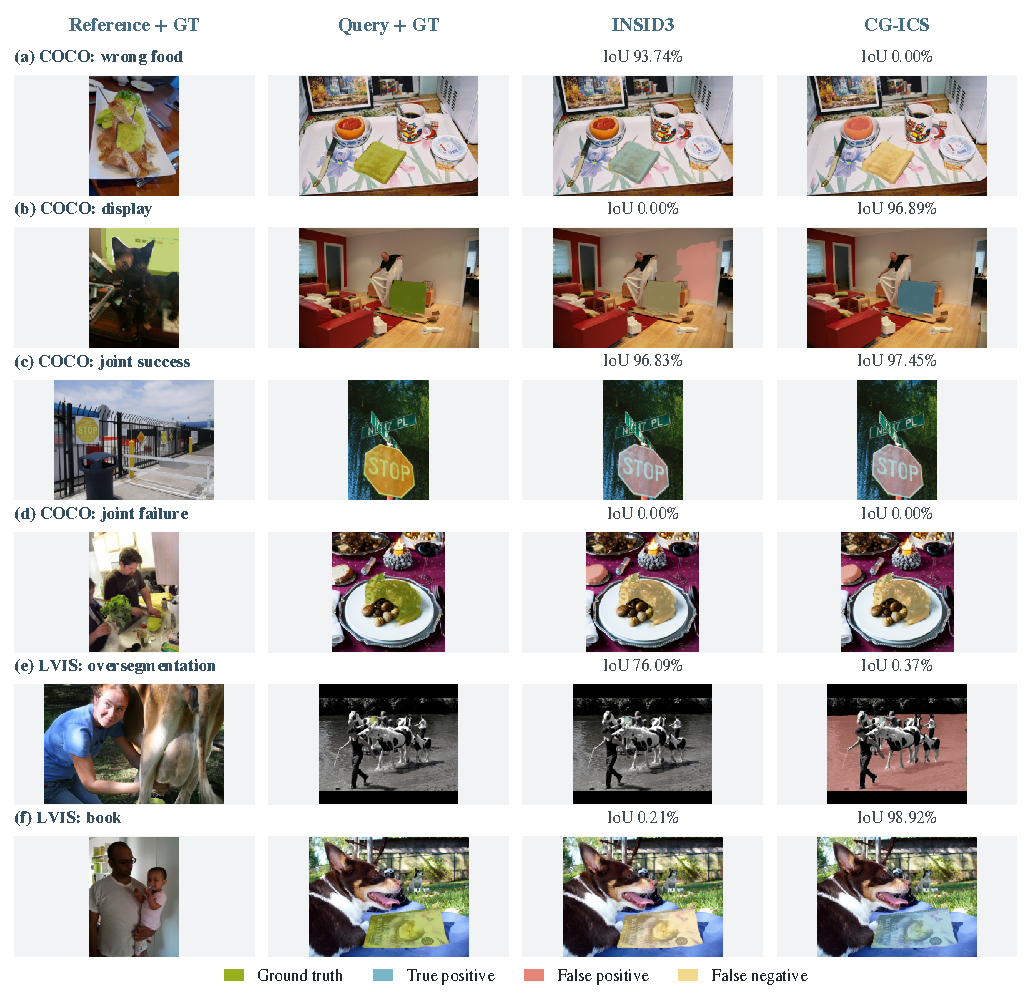
\includegraphics[width=0.92\linewidth]{figures/qualitative.pdf}
    \caption{\textbf{Complementary successes and failures.} Matched reference--query examples; colors indicate true positives, false positives, and false negatives.}
    \label{fig:qualitative}
\end{figure*}

\subsection{Parameter Sensitivity}
Single-factor sweeps show that increasing computation does not consistently improve accuracy. Raising the INSID3 clustering threshold from 0.6 to 0.7 decreases COCO equal-query IoU by 1.53 points but increases LVIS by 1.85. Reducing input size to 768 changes accuracy by $-0.88$ and $-2.25$ points while reducing matched latency to approximately 0.39--0.41 of the default.

For CG-ICS, using one initial candidate changes equal-query IoU by $-0.16$ points on COCO and $-0.82$ on LVIS; same-GPU matched latency is approximately 0.63--0.66 of the default. One search loop has little observed COCO penalty but reduces LVIS accuracy by 0.75 points. Accuracy effects use the full component cohort, while timing ratios use subsets with the same runner GPU model. Full intervals are in Appendix~\ref{app:cost}.

\subsection{Scale and Failure Analysis}
CG-ICS's accuracy advantage is largest on small query targets. For foreground area below 1\% of the image, its paired equal-query gain is 21.88 points on COCO and 24.03 on LVIS. The gain remains positive but smaller in the 1--10\% and at-least-10\% bins. Here size means semantic foreground proportion, measured on the query.



The examples in Figure~\ref{fig:qualitative} reveal complementary failure modes. CG-ICS recovers a book and monitor missed by INSID3. INSID3 succeeds on a food target for which CG-ICS selects a distractor under the concept \emph{salmon medallion}. Both methods accurately trace a stop sign, and both fail on another food target. A bowl example illustrates excessive background coverage.

Other inspected cases connect semantic specificity to the predicted region: \emph{floor unit} selects the floor rather than a vacuum cleaner, \emph{buttered bread} covers bread rather than the small butter target, and \emph{vehicle} includes a bus outside the prompted car regions. These cases motivate testing concept quality as well as mask quality.

Four additional failures occur during reference preprocessing. Three distinct reference masks contain only one or five foreground pixels, which disappear when resized to $512\times512$ by legacy nearest-neighbor sampling. CG-ICS then stops before model inference. These failures motivate foreground-preserving resizing. Together, the variable search gains, latency gap, and semantic errors suggest allocating concept search according to the input rather than applying the same search budget uniformly.


